\documentclass{article}
\usepackage{amsmath, amssymb, amsthm}
\usepackage{tikz}
\usetikzlibrary{matrix,arrows}

\begin{document}
	
	\textbf{1.} Let $X$ and $Y$ be topological spaces. We consider in $C(X, Y)$ (with the compact-open topology) the subspace $C$ of constant functions.
	
	\textbf{a)} Prove that if $X$ is locally compact and Hausdorff, then $C$ is a retract of $C(X, Y)$.
	
	\textbf{b)} Under the same hypotheses as the previous item, prove that if $X$ is contractible, then $C$ is a strong deformation retract of $C(X, Y)$.
	
	\textbf{2.} Let $p: E \rightarrow B$ be a covering map, where $B$ is path-connected and $E$ is simply connected. Let $b_0 \in B$, $e_0 \in p^{-1}(b_0)$, and $f: B \rightarrow B$ be a continuous function with $f(b_0) = b_0$. Recall the pullback
	
	\[ E' = E \times_{B} B = \{(e, b) \in E \times B : p(e) = f(b)\}, \]
	
	given by the diagram:
	\begin{center}
		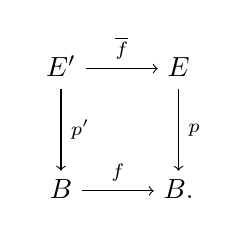
\begin{tikzpicture}[description/.style={fill=white,inner sep=2pt}]
			\matrix (m) [matrix of math nodes, row sep=3em,
			column sep=2.5em, text height=1.5ex, text depth=0.25ex]
			{ E' & E \\
				B & B. \\};
			\path[->,font=\scriptsize]
			(m-1-1) edge node[auto] {$ \overline{f} $} (m-1-2)
			(m-1-2) edge node[auto] {$ p $} (m-2-2)
			(m-1-1) edge node[right] { $p' $} (m-2-1)
			(m-2-1) edge node[auto] {$ f $} (m-2-2);
		\end{tikzpicture}
	\end{center}
	
	Prove that $p': E' \rightarrow B$ is a covering map, and $p'_*(\pi_1(E', (e_0, b_0)))$ is the kernel of $f_*: \pi_1(B, b_0) \rightarrow \pi_1(B, b_0)$.
	
	
\end{document}
